\section{Analysis}
\label{sec:analysis}

\subsection{Tight classes on labeled images do not reach the others}
\label{sec:geometry}

\paragraph{The diagnostic}
For a set of images $S$ with class labels, let $\mu_c$ be the mean encoder feature of class $c$ in $S$ and
$\sigma_c^2$ the mean squared distance of the features of class $c$ to $\mu_c$. The class-distance
normalised variance \citep{galanti2022role} of $S$ is
\begin{equation}
\label{eq:cdnv}
\mathrm{CDNV}(S) \;=\; \frac{1}{C(C-1)}\sum_{c\neq c'} \frac{\sigma_c^2+\sigma_{c'}^2}{2\,\lVert\mu_c-\mu_{c'}\rVert^2},
\end{equation}
the average over all ordered pairs of the $C$ classes; we compute it on the 512-dimensional encoder
features without normalisation. A small value means tight, well separated classes. We evaluate
\cref{eq:cdnv} on three disjoint sets, each with its own class means: the 5,000 \emph{labeled} training
images, the \emph{other} 45,000 training images, and the 10,000 \emph{test} images. The same three sets are
used for every method, so the numbers are comparable across methods. What differs is the role of the middle
set: \supcon, \simclrsub and cross-entropy on the 5,000 labels never see the other 45,000 images, while
\simclr and \union train on them without labels. The ground-truth labels of the 45,000 images are used only
for this measurement.

\begin{table}[t]
\centering
\small
\caption{Class tightness (CDNV, \cref{eq:cdnv}) on three sets of images, and accuracy of the \lpfive probe on
its own training images and on test images (CIFAR-10, 10\% labels, ResNet-18, 19,400 steps; mean $\pm$
standard deviation over seeds).}
\label{tab:geometry}
\begin{adjustbox}{max width=\linewidth}
% generated by scripts/make_assets.py -- do not edit
\begin{tabular}{lcccccc}
\toprule
 & \multicolumn{3}{c}{CDNV ($\downarrow$ tighter classes)} & & \multicolumn{2}{c}{LP-5k accuracy} \\
\cmidrule(lr){2-4}\cmidrule(lr){6-7}
encoder (19,400 steps) & labeled 5k & other 45k & test 10k & test / labeled & on its 5k & test \\
\midrule
\simclr & 1.58{\scriptsize$\,\pm\,$0.02} & 1.57{\scriptsize$\,\pm\,$0.01} & 1.61{\scriptsize$\,\pm\,$0.01} & 1.0 & 90.7{\scriptsize$\,\pm\,$2.3} & 85.8{\scriptsize$\,\pm\,$0.2} \\
\simclrsub & 6.12 & 5.80 & 5.64 & 0.9 & 80.9 & 69.2{\scriptsize$\,\pm\,$0.9} \\
\supcon & 0.23{\scriptsize$\,\pm\,$0.01} & -- & 0.68{\scriptsize$\,\pm\,$0.01} & 2.9 & 100.0{\scriptsize$\,\pm\,$0.0} & 81.5{\scriptsize$\,\pm\,$0.3} \\
\union & 0.51{\scriptsize$\,\pm\,$0.01} & -- & 1.64{\scriptsize$\,\pm\,$0.01} & 3.2 & 100.0{\scriptsize$\,\pm\,$0.0} & 80.7{\scriptsize$\,\pm\,$0.6} \\
cross-entropy on 5k & 0.00{\scriptsize$\,\pm\,$0.00} & 0.15{\scriptsize$\,\pm\,$0.01} & 0.16{\scriptsize$\,\pm\,$0.00} & 165.2 & 100.0{\scriptsize$\,\pm\,$0.0} & 83.5{\scriptsize$\,\pm\,$0.5} \\
\simclr{}$\to$\supcon & -- & -- & -- & -- & -- & 87.7{\scriptsize$\,\pm\,$0.3} \\
\bottomrule
\end{tabular}

\end{adjustbox}
\end{table}

\begin{figure}[t]
\centering
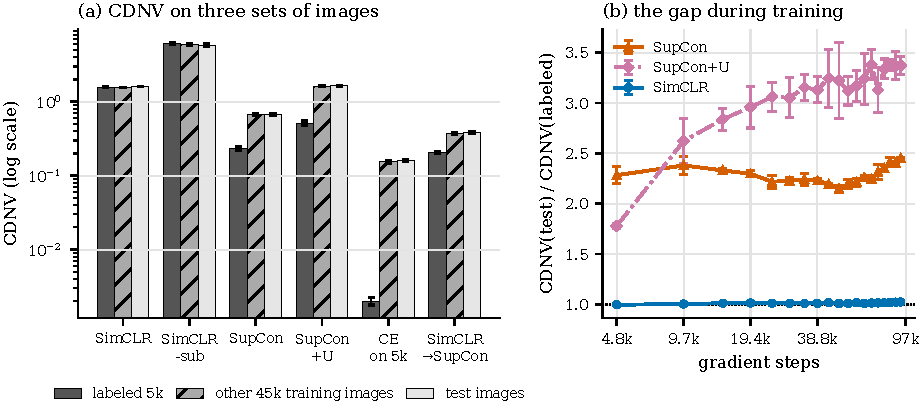
\includegraphics[width=\linewidth]{figures/fig_geometry.pdf}
\caption{(a) CDNV on the labeled images, on the other training images and on test images at 19,400 steps
(log scale, mean $\pm$ standard deviation over seeds). (b) Ratio of the CDNV on test images to the CDNV on
the images the method used with labels (\supcon, \union) or trained on (\simclr), during training.}
\label{fig:geometry}
\end{figure}

\paragraph{What the split shows}
\Cref{tab:geometry} and \cref{fig:geometry}(a) give three observations.

\emph{Label-free pretraining treats all images alike.} For \simclr the CDNV is the same on labeled images
(\R{simclr_all_e200:cdnv_lab}), other training images (\R{simclr_all_e200:cdnv_rest}) and test images
(\R{simclr_all_e200:cdnv_test}).

\emph{\supcon is tight where it had labels.} Its CDNV is \R{supcon_lab_f0.1_e200:cdnv_lab} on the labeled
images and \R{supcon_lab_f0.1_e200:cdnv_test} on test images, a ratio of
\R{supcon_lab_f0.1_e200:cdnv_ratio}. The other 45,000 training images, which it never saw, behave like test
images (\R{supcon_lab_f0.1_e200:cdnv_rest}).

\emph{In \union the labels do not spread.} \union trains on all 50,000 images, yet its CDNV is
\R{union_f0.1_e200:cdnv_lab} on the labeled 5,000 and \R{union_f0.1_e200:cdnv_rest} on the 45,000 images it
saw without labels, which is as loose as on test images (\R{union_f0.1_e200:cdnv_test}) and as loose as
\simclr. The joint loss makes the labeled images tight and leaves the unlabeled ones where instance
discrimination puts them. This is the direct reason why \union looks good to a probe that brings fresh
labels for the 45,000 images and gains nothing for a probe restricted to the 5,000.

\paragraph{The gap is not specific to \supcon}
Cross-entropy training on the 5,000 labels shows the same pattern in a stronger form: the labeled images
collapse almost completely (CDNV \R{ce_f0.1_e200:cdnv_lab}) while test images stay at
\R{ce_f0.1_e200:cdnv_test}. The gap between seen and unseen images is therefore ordinary supervised
overfitting to a small labeled set, as described for neural collapse by \citet{hui2022limitations}, and not
a property of the contrastive loss. What is specific to the label-scarce contrastive setting is its
consequence: the labels have been used to fit 5,000 images, and reusing them in a probe or in fine-tuning
adds little. Cross-entropy on the 5,000 labels is in fact tighter on test images than \supcon
(\R{ce_f0.1_e200:cdnv_test} against \R{supcon_lab_f0.1_e200:cdnv_test}) and slightly more accurate
(\cref{tab:where}).

\paragraph{Dynamics}
\Cref{fig:geometry}(b) follows the ratio between the CDNV on test images and on the labeled images during
the longest runs for which it was logged (\R{geomcurve:supcon:n} seeds, checkpoints up to
\R{geomcurve:supcon:laststep} steps). For \supcon the ratio is already
\R{geomcurve:supcon:first} at \R{geomcurve:supcon:firststep} steps, when its accuracy has almost stopped
improving, and keeps rising to \R{geomcurve:supcon:last}; for \union it rises from \R{geomcurve:union:first}
to \R{geomcurve:union:last}; for \simclr, measured between all training images and test images, it stays at
\R{geomcurve:simclr:last}. The labeled images keep getting tighter relative to new images while the accuracy
no longer improves. This is consistent with the plateau of \supcon being reached once the labeled images are
fitted; the evidence is correlational and we do not claim more.

\subsection{Does the coverage of the labeled pool explain the limit of \supcon?}
\label{sec:coverage}
A natural hypothesis is that \supcon on a small pool is limited by how well the pool \emph{covers} the data:
low-budget active learning and data pruning find that coverage is what matters for small sets
\citep{hacohen2022active,yehuda2022active,sorscher2022beyond}. We test it with an intervention that keeps
the pool size at 5,000 images (500 per class) and changes only which images are in it.

\paragraph{Pools and statistics}
Features are taken from a reference encoder and $\ell_2$-normalised. For a pool $S$, the \emph{coverage
radius} is the mean, over test images $x$, of the cosine distance from $x$ to the nearest pool image of the
same class; the \emph{spread} is the mean cosine distance between two pool images of the same class. Both
are averaged over classes (formulas in \cref{app:pools}). We build three families of pools: random; mixtures
in which 25, 50, 75 or 100\% of each class is chosen by greedy $k$-center selection \citep{sener2018coreset},
which favours atypical images, and the rest at random; and mixtures in which 25, 50, 75 or 100\% consists of
groups of 50 near-duplicates in feature space (``redundant''), and the rest at random. Each pool is drawn
for three seeds, and \supcon and \simclr are trained on it for 9,700 steps. To check that the result does
not depend on measuring distances with a \simclr encoder, all statistics are computed in two reference
spaces: a \simclr encoder trained on all images and a supervised encoder trained on all labels.

\begin{figure}[t]
\centering
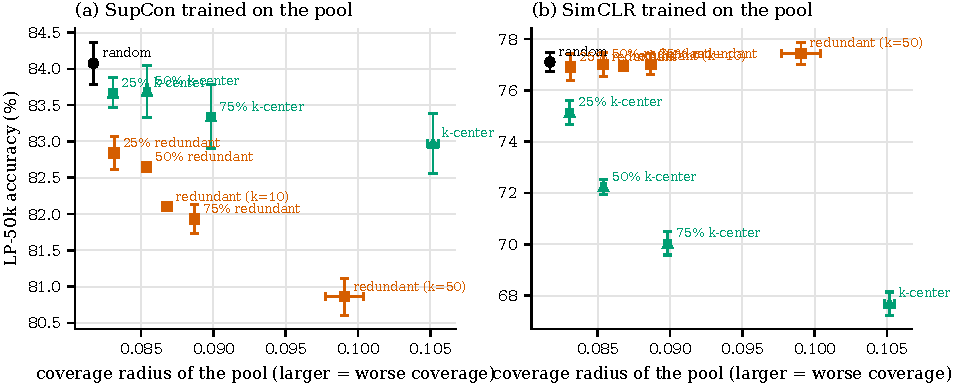
\includegraphics[width=\linewidth]{figures/fig_coverage.pdf}
\caption{Accuracy of (a) \supcon and (b) \simclr trained for 9,700 steps on pools of 5,000 images with
different coverage (CIFAR-10; mean $\pm$ standard deviation over seeds; coverage radius in the \simclr
reference space). Black: random pool; green: mixtures with $k$-center selection; red: mixtures with redundant
groups.}
\label{fig:coverage}
\end{figure}

\paragraph{Result}
\pending{Within the redundant family the picture is clean: as the share of near-duplicates grows, the
coverage radius grows and the accuracy of \supcon falls monotonically, from \R{supcon_lab_f0.1_e100:lp50}\%
for the random pool to \R{supcon_lab_cluster50_f0.1_e100:lp50}\% for the fully redundant one. The
$k$-center family behaves differently: its coverage radius is the largest of all pools, yet \supcon loses
little accuracy (\R{supcon_lab_kcenter_f0.1_e100:lp50}\%), while \simclr trained on the same pool collapses
(\R{simclr_sub_kcenter_f0.1_e100:lp50}\%). Across all pools the rank correlation between coverage radius and
the accuracy of \supcon is \R{rho:all:radius_simclr:supcon} (Spearman, $n=\R{rho:all:radius_simclr:supcon:n}$
pools); within the random and redundant pools it is \R{rho:nokc:radius_simclr:supcon}. The supervised
reference space gives \R{rho:all:radius_supervised:supcon} and \R{rho:nokc:radius_supervised:supcon}. Across
pool sizes from 1\% to 20\%, the partial rank correlation that controls for the pool size is
\R{rho:partial}.} The $k$-center pool is the kind of set that \citet{hacohen2022active} show to be a poor
choice at low budgets for \emph{supervised} learners; here the labels make \supcon robust to it, and the
label-free learner is the one that fails. $k$-center selection picks the images farthest from all others,
that is, atypical images and outliers. Without labels, each of them has few similar images in the pool, so
instance discrimination learns features specific to single images; with labels, the atypical images of a
class are positives of each other, and the class-level positives bridge the gaps between them.

We conclude that coverage explains part of the effect of pool composition, namely the cost of redundancy,
and that no single statistic of the pool predicts the accuracy of both learners. Spread, a natural
candidate, does not separate pools of different size (it is flat from 1\% to 100\% of the data,
\cref{app:pools}) and ranks the $k$-center pool best; it does decrease with redundancy, in line with the
accuracy of \supcon.

\subsection{Labels make colour augmentation less necessary}
\label{sec:jitter}
\simclr is known to depend on colour distortion: without it, two crops of an image can be matched by their
colour histogram alone \citep{chen2020simclr,chen2021intriguing,robinson2021can}. Labels offer another way
out of this shortcut, because two different images of a class do not share a histogram. \Cref{tab:jitter}
removes colour jitter (keeping random grayscale) from the three methods. \simclr loses
\R{jitter:simclr_all_e100}\pt, and \supcon only \R{jitter:supcon_lab_f0.1_e100}\pt. \union loses \R{jitter:union_f0.1_e100}\pt, in between: only the quarter of each batch that is labeled has
class positives, while the unlabeled three quarters are trained by instance discrimination and are exposed to
the colour shortcut like \simclr. Where good augmentations are not
known, for example outside natural images, this is an argument for using labels in the loss that our
accuracy comparison does not capture. The full analysis of colour reliance in \simclr is in
\cref{app:colour}.

\begin{table}[t]
\centering
\small
\caption{Removing colour jitter from the augmentation (CIFAR-10, 10\% labels, 9,700 steps, \lpall accuracy
in \%, mean $\pm$ standard deviation over seeds; the change is computed per seed).}
\label{tab:jitter}
% generated by scripts/make_assets.py -- do not edit
\begin{tabular}{lcccc}
\toprule
method & seeds & full augmentation & without colour jitter & change \\
\midrule
\simclr & 1 & 83.9 & 77.1 & -6.8 \\
\supcon & 1 & 84.0 & 82.7 & -1.3 \\
\bottomrule
\end{tabular}

\end{table}
